\chapter{Preparation of Datasets}
\label{chap:preparations data sets}
% Todo: 6 pages?

Next to the ML model selected, the data used to train and evaluate the model has a major influence on its performance. If the data is not representative or information is missing about the underlying process that the model should be fitted to, there can be errors, bias, or an inability to generalize well to new data. In this chapter, we look at potential features for air temperature, at data sources for these features, and discuss the construction process of the datasets used in this work.\\
% Overall dataset availability
In the field of natural language processing (NPL) and computer vision (CV), there is an abundance of large available datasets which have a big contribution to the advancements in the field, like annotated datasets as provided by Google Research~\footnote{\url{https://research.google/resources/datasets/}, \textit{last accessed: 05.08.2023}}. In comparison in the field of climate research, there are also many datasets, including satellite data, weather station data, and climate model data, however they are highly distributed or often not openly available. Platforms such as Google Earth Engine~\cite{gorelick2017google} try to address this issue, however the dataset catalogue~\footnote{\url{https://developers.google.com/earth-engine/datasets}, \textit{last accessed: 05.08.2023}} is still limited and does not include datasets offered by local authorities or other research institutions, such as universities.\\
% How does the perfect dataset for air temperature look like?
For the specific use case of temperature interpolation in urban areas, an optimal dataset would contain high spatial and temporal resolution sensor data, e.g., a high sensor density and a low time interval of for example five to ten minutes. Additionally, the sensor placement and sensor quality have a high influence on the accuracy of the sensor readings~\cite{oke2006guideline}, therefore the correct placement and calibration of the sensors needs to be guaranteed. Such requirements are not met by traditional weather station networks as the spatial coverage is too low, as a single weather station is not enough to capture the urban microclimate~\cite{oke2017urban}. The weather station locations of the DWD are shown in figure~\ref{fig:dwd sensor locations germany}, which shows that usually at most one weather station is available per city. The weather stations however offer a high temporal resolution in addition to very high-quality sensors, which is why they can be used as reference stations for quality control of other sensors, as discussed in section~\ref{sec:quality control}.\\
A solution to the problem of low spatial coverage is the usage of sensor networks. There are several projects that run dense urban-climate monitoring networks~\cite{muller2013sensors} such as the Helsinki Testbed~\cite{koskinen2011helsinki} or the Birmingham Urban Climate Laboratory~\cite{warren2016birmingham}, however access to those datasets is limited, for example due to outdated links or the need to request access. Due to the high cost of running such dense sensor networks with high sensor and maintenance costs, professionally run sensor networks are rare and are often only run for a limited period until project funds run out.\\
As an alternative, sensor networks can also be crowdsourced and run by citizens, distributing the cost of individual sensors as well as maintenance costs among many. Especially with advances in sensor technologies, lost cost and compact sensors are more affordable than ever while still providing good data quality~\cite{grimmond2006progress, rundel2009environmental}. In the context of meteorological data, such sensor networks are often referred to as citizen weather station (CWS)~\cite{meier2017crowdsourcing} or personal weather station (PWS)~\cite{hahn2022observations} networks. In this work, we use the term PWS.\\
The main downside of this approach is the lack of quality control and meta data, as the sensors are usually placed by non-professionals in suboptimal locations, e.g., in direct sunlight or too close to walls, leading to incorrect readings or bias in the data. A lack in meta data can also lead to issues, if for example exact positions of the sensors are not known and information about the height of the sensor above ground is missing. However, other concerns such as data privacy also need to be accounted for, as such weather stations are often placed on private property.\\
In this work, data from PWS networks is used to create datasets for the training and evaluation of ML models for air temperature interpolation. In the following sections, we look at available PWS providers and their data and potential features for air temperature interpolation, discuss additional pre-processing steps such as quality control or sensor height correction, and finally discuss the construction of the datasets used in this work.

\section{Private Weather Station Network Providers}
\label{sec: private weather station network providers}

PWS providers offer a platform for users to upload their sensor data and either sell weather stations and sensors themselves (e.g., Netatmo) or provide guides to allow users to connect their own sensors to the platform (e.g., Sensor.Community). Netatmo data in particular has been used in several studies~\cite{meier2017crowdsourcing, hahn2022observations, venter2020hyperlocal, zumwald2021mapping} and has seen complementary studies for example discussing QC\\
processes~\cite{fenner2021crowdqc+}, later seen in Section~\ref{sec:quality control}. There are also other PWS network providers such as Sensor.Community or Weather Underground (WOW) that have been used in several studies~\cite{ho2014mapping}. To find out which provider best fits our needs in this work, the following section compares the different providers and their data.

\subsection{Sensor.Community}

Sensor Community~\footnote{\url{https://sensor.community/en/}, \textit{last accessed: 05.08.2023}} is a contributors driven global sensor community that creates Open Environmental Data and has an archive~\footnote{\url{https://archive.sensor.community/}, \textit{last accessed: 05.08.2023}} of their historical sensor data world-wide. There are no quality measures recorded for each sensor, but as crowd-sourced sensor data tends to have a lower quality than professionally setup sensors, e.g., sensor placement by non-professionals, we need to explore how the data quality looks like.
In Figure~\ref{fig:temperature_sensor_community_map}, where we see the greater Hamburg area with a currently reported temperature of 25°C by the DWD Fuhlsbüttel station, there are multiple sensors that report a temperature of 30°C and above, which could be either due to the sensor being placed in direct sunlight or due to the sensor being faulty. An outlier near Pinneberg is shown in Figure~\ref{fig:temperature_sensor_community_outlier}, where one sensor reports 25°C, as currently expected, and one sensor reporting 50°C, which is clearly an outlier. This data quality issue needs to be addressed in the data pre-processing step and can result in a significant reduction of available data. This was also an issue discussed in~\cite{meier2017crowdsourcing}, as ``erroneous metadata, failure of data collection, and unsuitable exposure of sensors lead to a reduction of data availability by 53 \%``.
From a meta-data perspective, there is no information on the sensor height above ground as well as no quality measures for each sensor, or information on the sensor location accuracy.

\begin{figure}[ht]
    \centering
    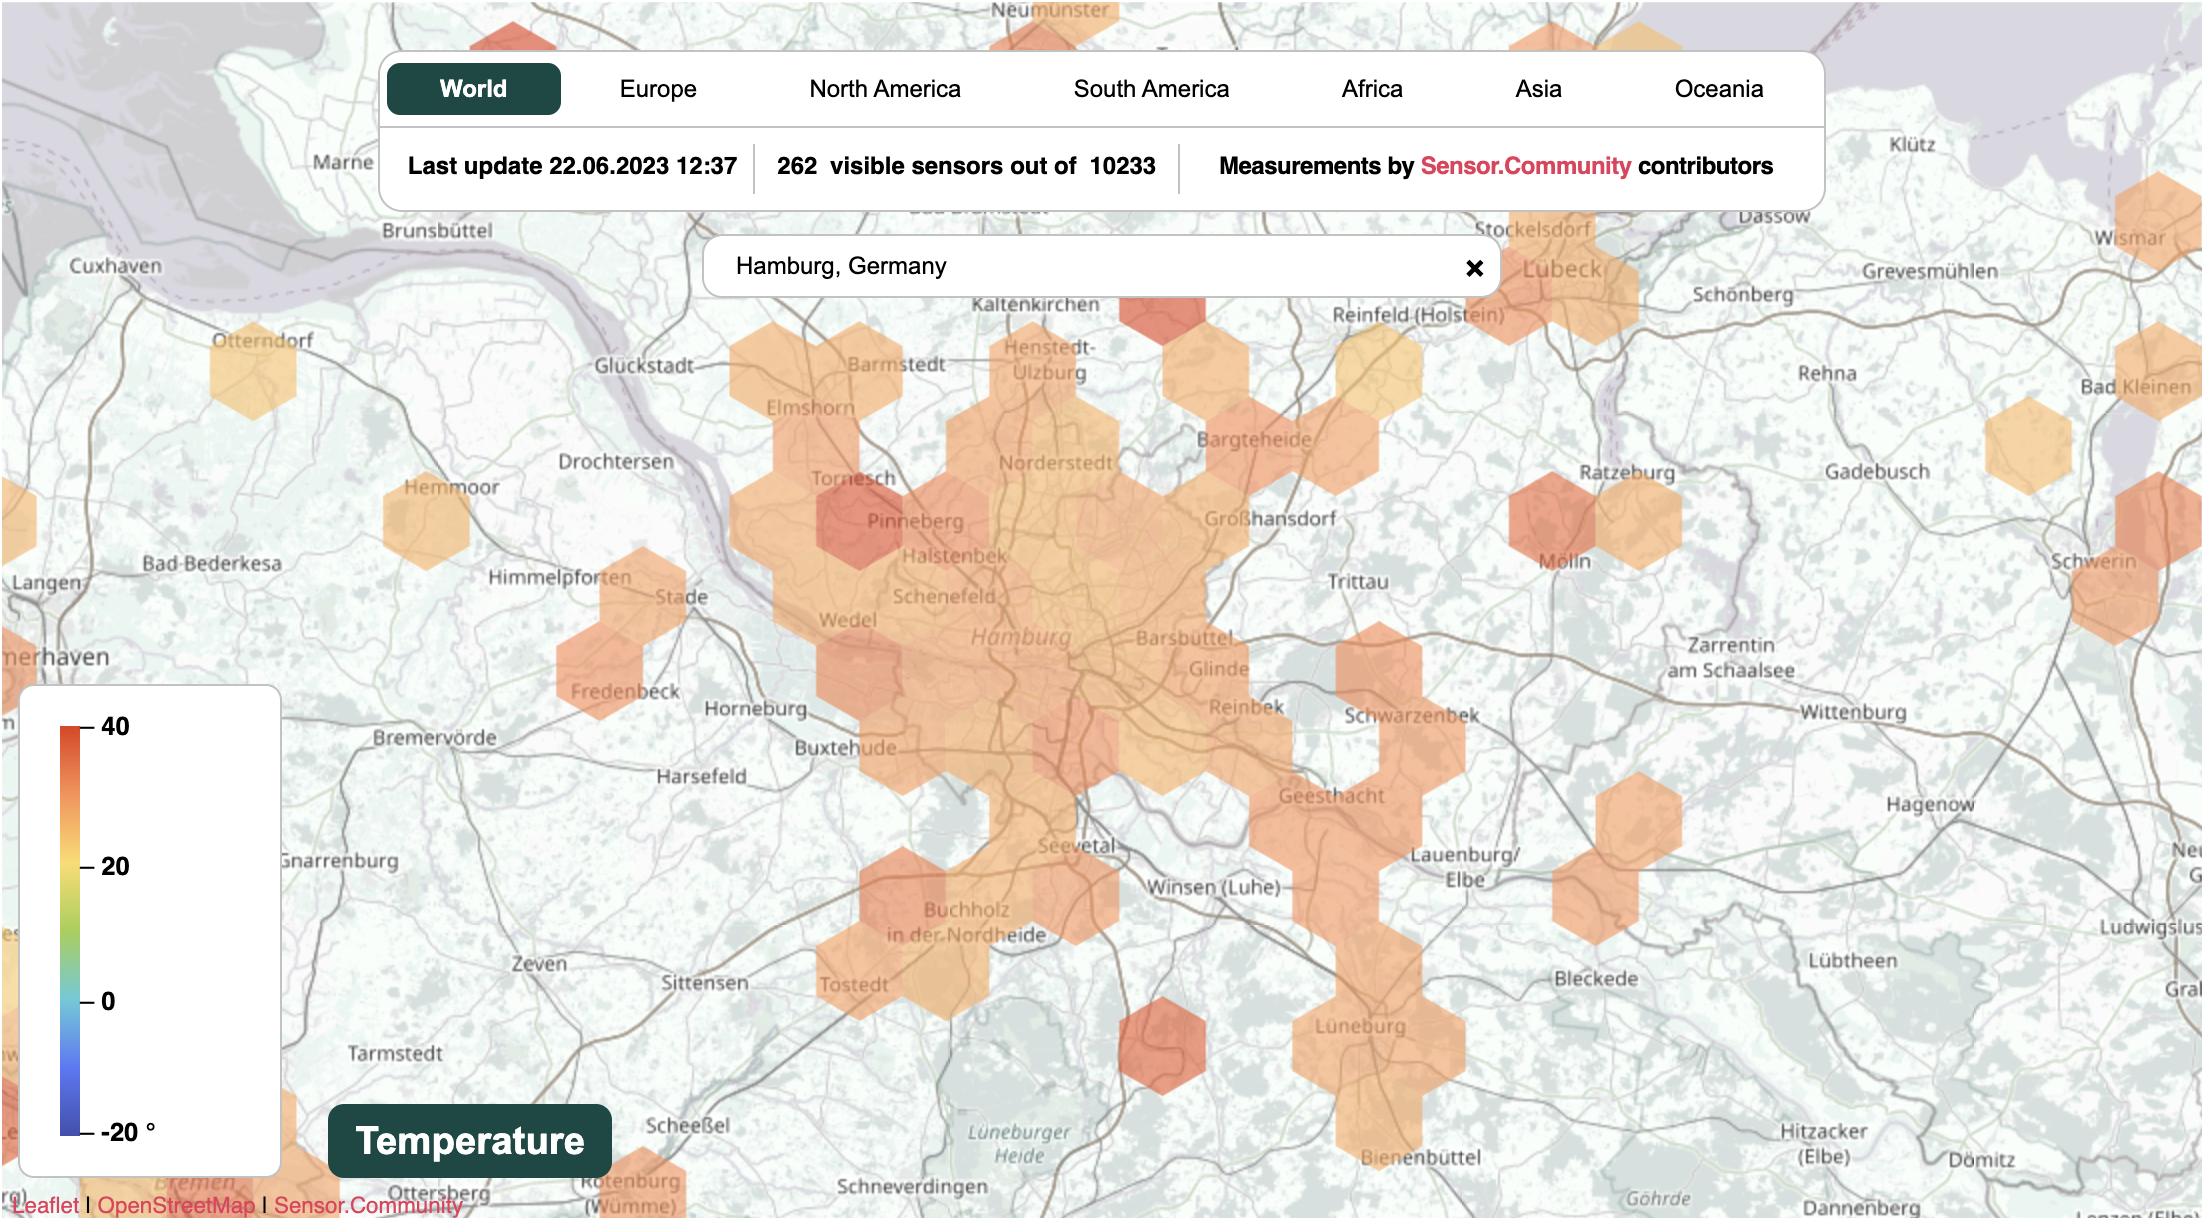
\includegraphics[width=1\textwidth]{images/sensor_community_temperature_map.png}
    \caption{Temperature map from Sensor Community for Hamburg, Germany, on 22.06.2023 12:51h with the DWD reference at 25°C}
    \label{fig:temperature_sensor_community_map}

    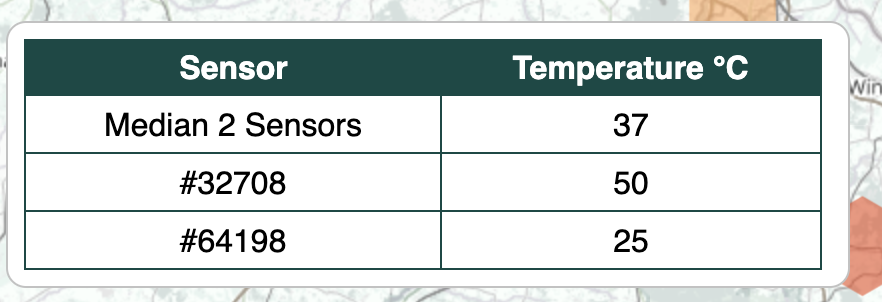
\includegraphics[width=0.8\textwidth]{images/sensor_community_outliers.png}
    \caption{Temperature outlier from Sensor Community for Hamburg, Germany, on 22.06.2023 12:51h with the DWD reference at 25°C}
    \label{fig:temperature_sensor_community_outlier}
\end{figure}

Overall, there are around 11.738 active sensors~\footnote{as of 24.06.2023}. Of these sensors, many are located in Germany, as seen in Appendix~\ref{sensor_community_sensors_by_countries}, and almost half of them are of type BME 280, which is a lost-cost Bosch sensor which can measure temperature, pressure, and humidity. The sensor locations as of May 2023 are shown in~\ref{fig:sensor community sensor locations germany}. DHT22 sensors can measure temperature and humidity, BMP280 and BMP180 sensors can measure temperature and pressure, and BME280 sensors can measure temperature, pressure, and humidity.\\

\begin{figure}[ht]
    \centering
    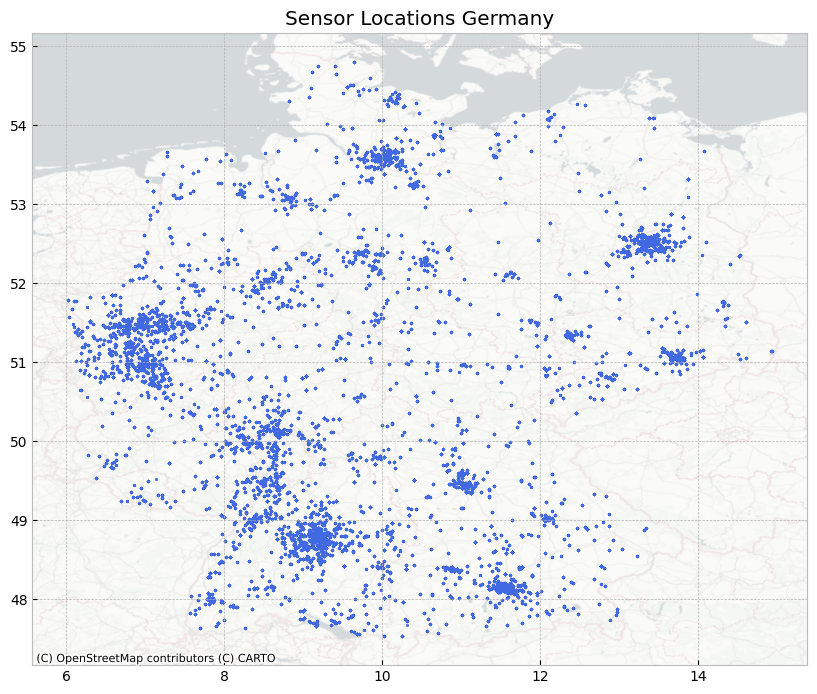
\includegraphics[width=1\textwidth]{images/sc_sensor_locations_germany.png}
    \caption{Sensor locations of Sensor Community in Germany, as of 01.05.2023, of sensor type DHT22 (2590 sensors), BME280 (1558 sensors), BMP280 (100 sensors), BMP180 (72 sensors)}
    \label{fig:sensor community sensor locations germany}
\end{figure}

\subsection{Netatmo}

Netatmo~\footnote{\url{https://www.netatmo.com/en-eu}} is a French company that sells smart-home devices including outdoor weather stations, indoor sensors for air quality, as well as other products such as smart cameras. They host a weather map~\footnote{\url{https://weathermap.netatmo.com/}, \textit{last accessed: 06.08.2023}} where customers can share their outdoor weather station data. They provide an API to access current weather station data as well historic data from individual outdoor sensors and modules.
They provide their historical and current weather data for commercial partners or partners in the research and education sector. They are part of the EUMETNET project~\footnote{\url{https://www.eumetnet.eu/}, \textit{last accessed: 06.08.2023}} which is a network of 31 European meteorological and hydrological services (NMHSs). The project aims to facilitate the exchange of weather data and to improve the quality of weather forecasts, especially in the context of PWS~\cite{hahn2022observations}. There are currently no openly historical datasets available from Netatmo data, only private datasets~\footnote{\url{https://catalogue.ceda.ac.uk/uuid/e8793d74a651426692faa100e3b2acd3}, \textit{last accessed: 06.08.2023}} that are only available for partners such as EUMETNET members. They offer an educational program~\footnote{\url{https://www.netatmo.com/en-eu/weather-with-netatmo}} to access temporally and spatially limited amounts of data that is usually only available to commercial partners.

% precisions
% Please add the following required packages to your document preamble:
% \usepackage{booktabs}
\begin{table}[]
\begin{tabular}{@{}lllll@{}}
\toprule
Measurement    & Unit    & Measurement Range      & Precision  & Recording Frequency              \\ \midrule
Temperature    & °C      & -40°C to 65°C          & 0.3°C   & averaged over 5 min              \\
Humidity       & \% (RH) & 0 to 100\%             & 3\%     & -                                \\
Air Pressure   & mbar    & 260 to 1160 mbar       & 1mbar   & -                                \\
Noise          & dB      & 35 to 120 dB           & -       & -                                \\
Wind Speed     & m/s     & 0 to 45 m/s (160 km/h) & 0.5 m/s & every 6 sec, averaged over 5 min \\
Wind Direction & °       & 0 to 359°              & 5°      & every 6 sec, averaged over 5 min \\
Rainfall       & mm/h    & 0.2 to 150 mm/h        & 1mm/h   & every 5 min (bucket is emptied)  \\ \bottomrule
\end{tabular}
\caption{Netatmo Sensor Specifications (Vendor reported)}
\label{tab: netatmo sensor specs}
% todo: adjust to page size, maybe move to dataset chapter
\end{table}

In the context of collecting meteorological data, the smart weather products are of particular interest. These include a smart outdoor weather station that collects air temperature, humidity and air pressure, an anemometer that collects wind speed and direction, and a rain gauge. The sensor specifications, as reported by the vendor himself, is reported in Table~\ref{tab: netatmo sensor specs}.\\
In this work, data from Netatmo stations is used as Netatmo offers many sensors in Germany in urban areas, exemplified by Figure~\ref{fig:netatmo sensor locations hamburg} for the region of Hamburg, and by Figure~\ref{fig:netatmo sensor locations stuttgart} for the region of Stuttgart.
The developer portal~\footnote{\url{https://dev.netatmo.com/apidocumentation}} offers a way to programmatically access all public sensor measurements via a REST API, however each request has a limit on the spatial extend of the requested area for the current weather data. For historic data, the limit per request per sensor is 1024 data points. The API has a tight rate limit per application. For applications below 100 users, the rate limit is 2000 requests every hour and 200 requests every 10 seconds across all users, and 500 requests every hour and 50 requests every 10 seconds per user~\footnote{\url{https://dev.netatmo.com/guideline\#rate-limits}, \textit{last accessed: 06.08.2023}}. In this work, we use the REST API to collect sensor data from Netatmo sensors.

\begin{figure}[htp]
    \centering
    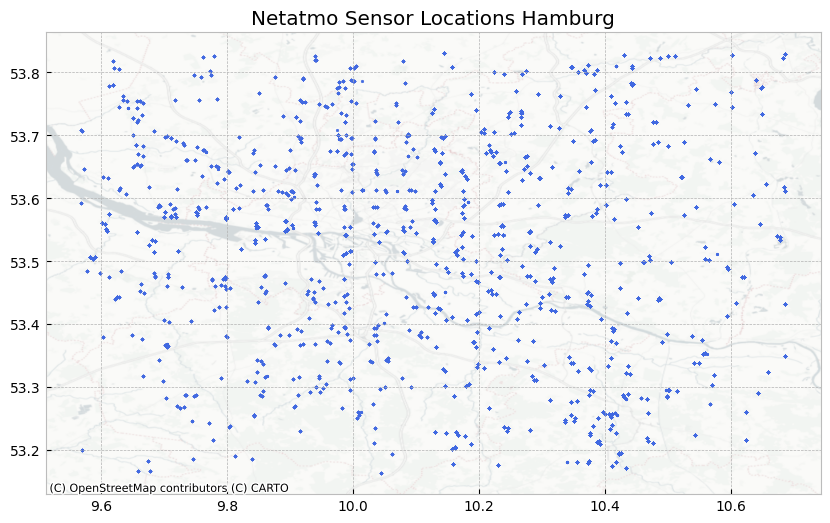
\includegraphics[width=1\textwidth]{images/netatmo_sensor_locations_hamburg.png}
    \caption{Sensor locations of Netatmo in Hamburg, Germany, as of 28.06.2023}
    \label{fig:netatmo sensor locations hamburg}

    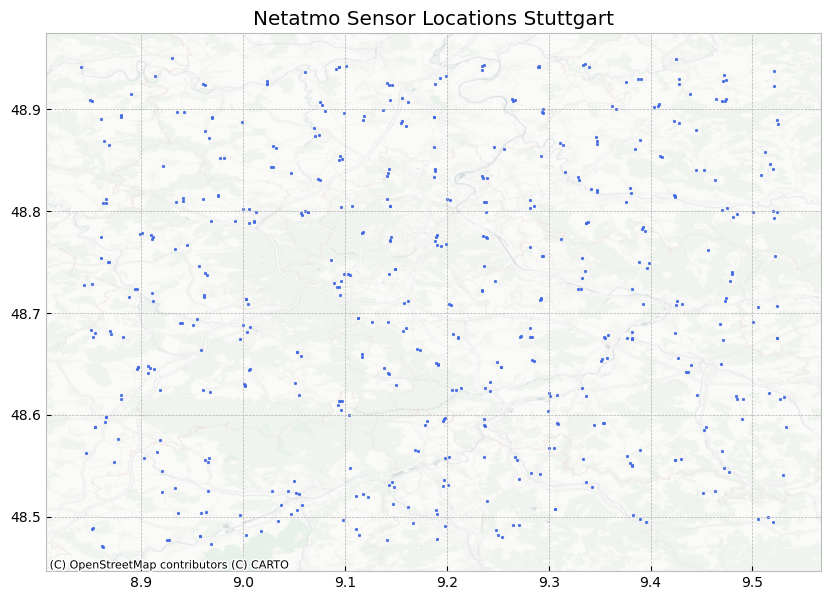
\includegraphics[width=1\textwidth]{images/netatmo_sensor_locations_stuttgart.png}
    \caption{Sensor locations of Netatmo in Stuttgart, Germany, as of 19.06.2023}
    \label{fig:netatmo sensor locations stuttgart}
\end{figure}

\subsubsection{Quality Considerations}

Netatmo sensors have a good measurement accuracy, however due to the compact design, an aluminium housing, poor ventilation due to the small case, no dedicated radiation screen resulting in a proneness to radiative errors, and therefore overall slow sensor-response time~\cite{meier2017crowdsourcing, buchau2018modelling}, Netatmo weather stations have a systematic bias that influences data quality. Due to the uniformity of Netatmo sensors, e.g., all sensors are built in the same way, this bias could be corrected in the QC step, however this is not further explored in this work.

\subsection{Other Providers}

Other sources for crowdsourced weather station data include Weather Observations Website (WOW)~\footnote{\url{https://wow.metoffice.gov.uk/}} and Weather Underground~\footnote{\url{https://www.wunderground.com/}}.
WOW is a platform run by the UK Met Office, which is the UK's national weather service, and has a dense sensor coverage in the UK and the Netherlands as seen in figure~\ref{fig:wow sensor locations}.
Weather Underground is a commercial weather service which also provides a crowdsourced weather station network. Unfortunately, Weather Underground only provides an API for users with a registered weather station or other bulk download options for historical data. The website would allow for manual download of historical data, but this is not feasible for the amount of data needed in this work.

\begin{figure}[ht]
    \centering
    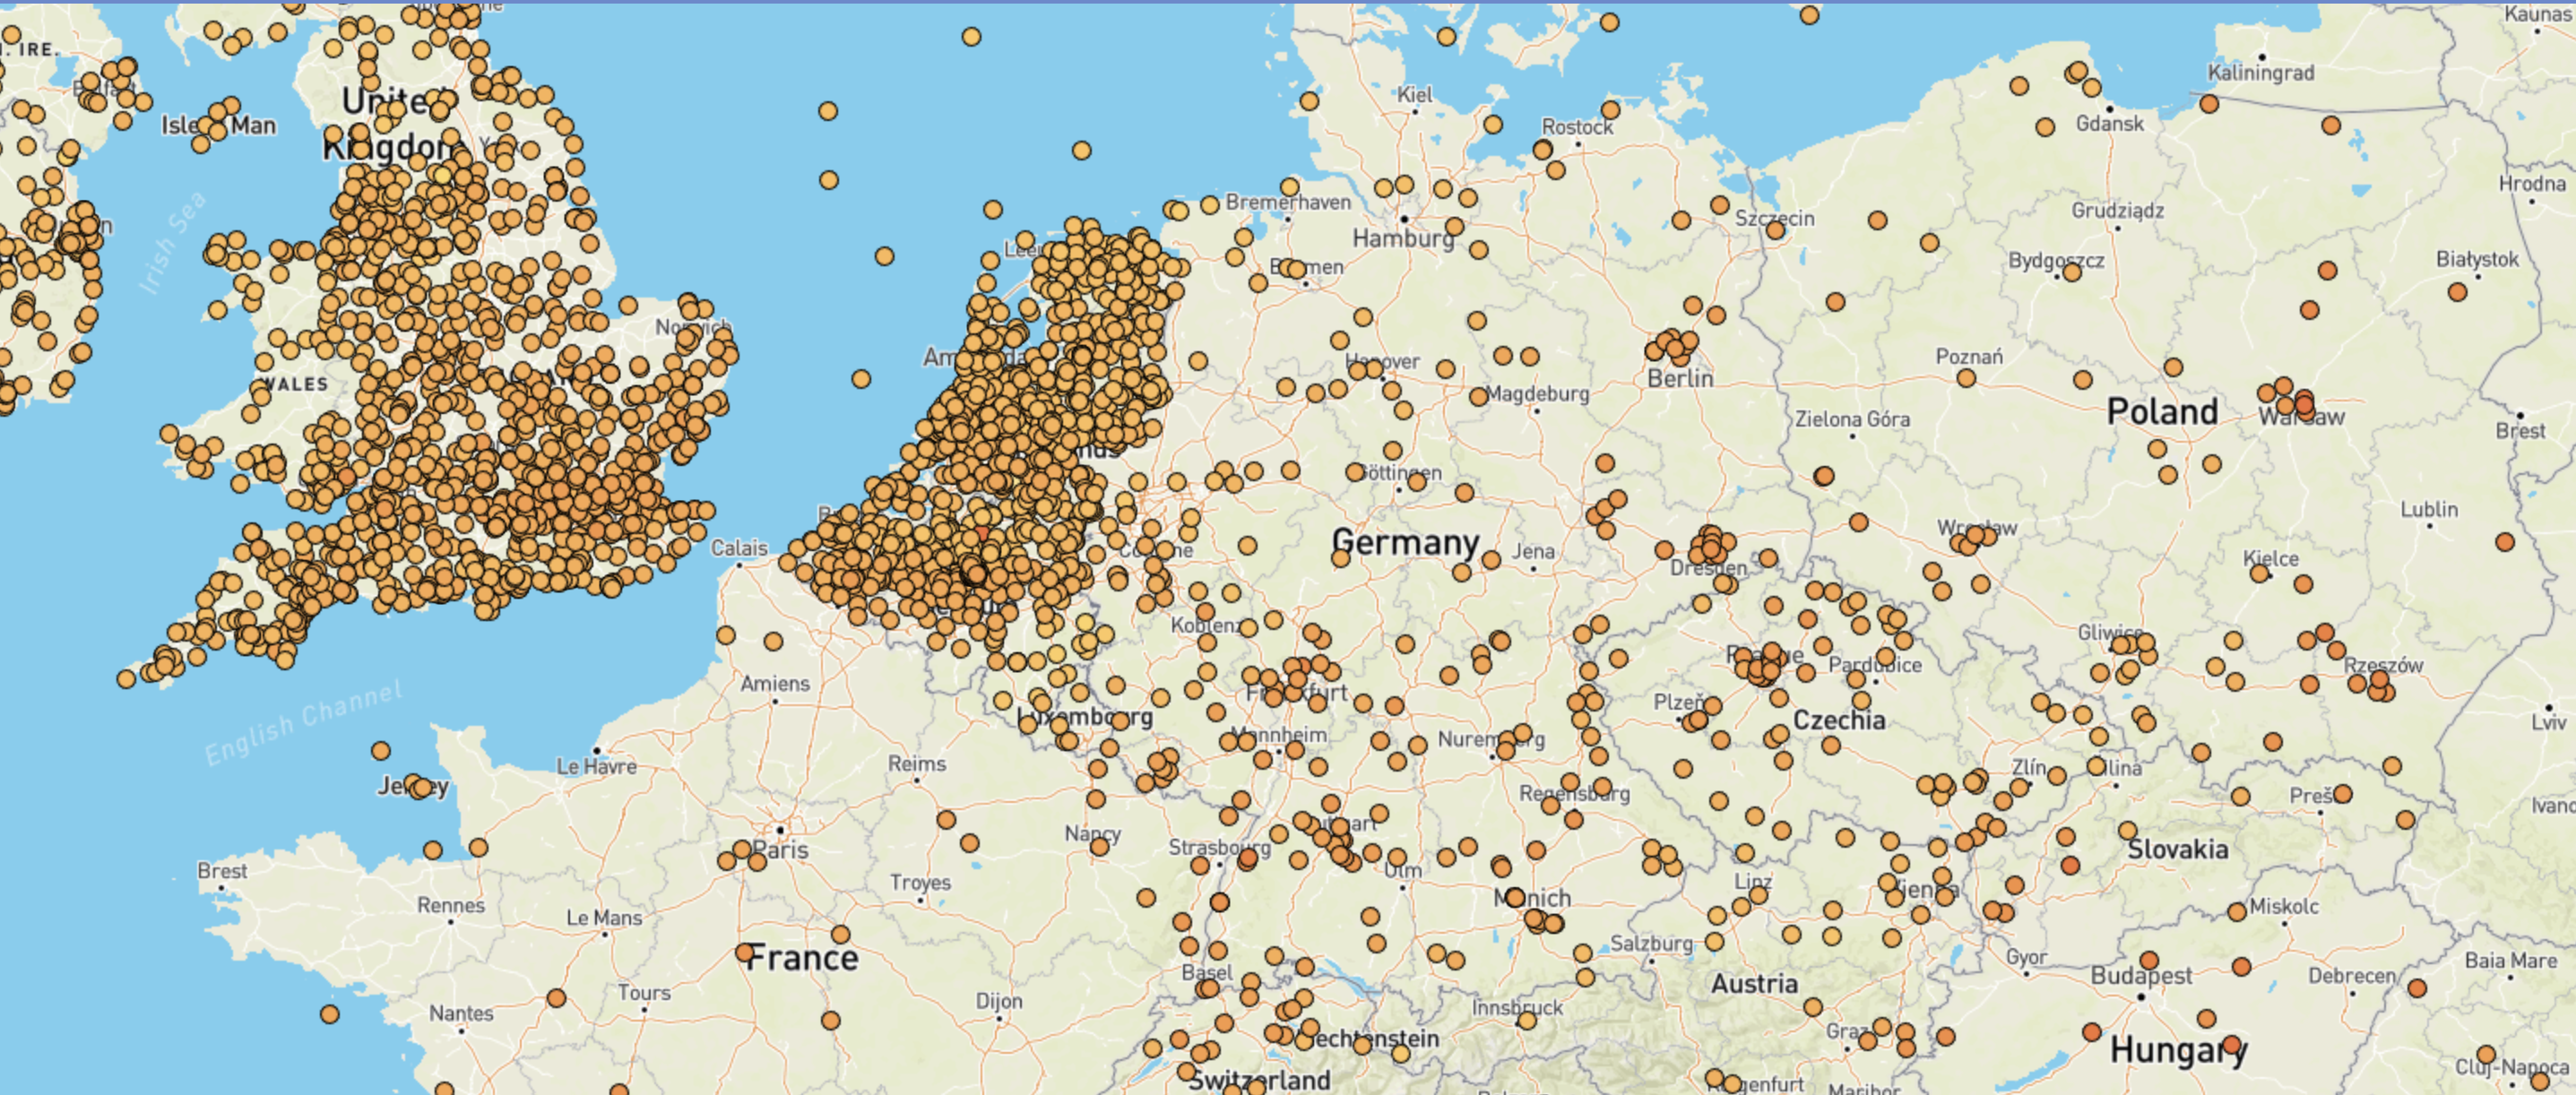
\includegraphics[width=1\textwidth]{images/wow_sensor_locations.png}
    \caption{Temperature sensor locations from WOW, accessed on 05.07.2023}
    \label{fig:wow sensor locations}
\end{figure}

\section{Reference Data Providers}

In order to add additional validation to crowdsourced weather data, reference data from (official) weather stations can be used. These weather stations should be setup according to current World meteorologicalOrganization (WMO) guidelines~\cite{wmo2018guide} to ensure high data quality. These standards are either achieved by official weather services, or by institutions such as universities whose sensors are maintained by experts.

\subsection{DWD}

The official German weather service (DWD) has many objectives that are defined by the DWD-law in Germany. Its tasks include meteorological and climatological monitoring of the atmosphere, meteorologically securing the airspace for civil aviation, monitoring the Maritim climate, and more. The DWD operates a large monitoring network and publishes most of its data via its OpenData portal~\footnote{\url{https://opendata.dwd.de/}, last accessed 13.07.2023}.\\
The main advantages of the DWD data are high data quality through reference instruments and proper setup according to WMO guidelines~\cite{wmo2018guide}. The main disadvantage is the low spatial coverage of the data, as stations are sparsely distributed to measure the overall mesoscale climate, as seen in Figure~\ref{fig:dwd sensor locations germany}. Additionally, a lot of the public weather stations are located close to airports, which are usually located outside of cities, and therefore not suitable for measuring urban microclimates.

\begin{figure}[ht]
    \centering
    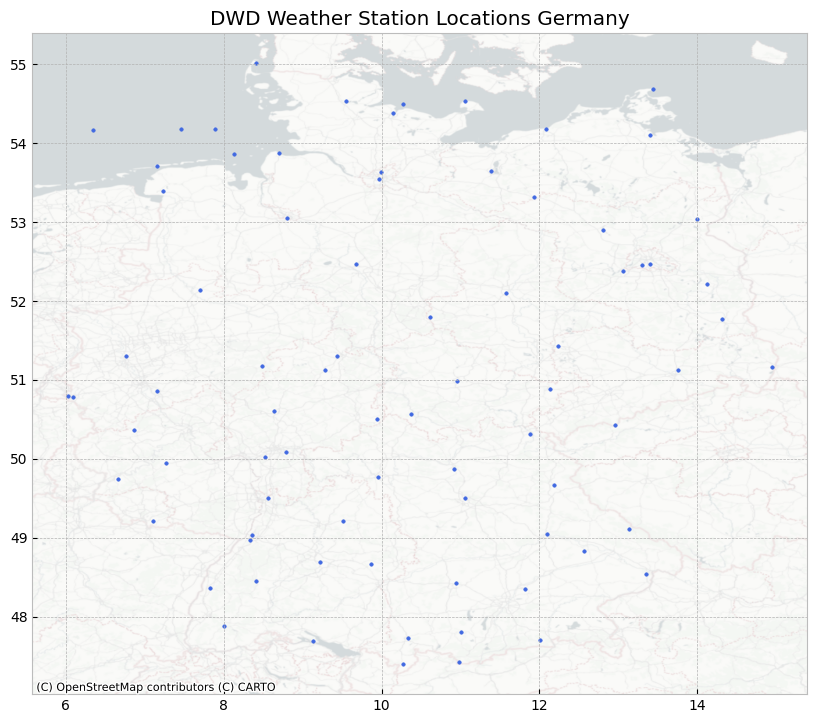
\includegraphics[width=1\textwidth]{images/dwd_weather_station_locations_germany.png}
    \caption{DWD Weather Station Locations in Germany, \url{https://opendata.dwd.de/climate_environment/CDC/observations_germany/climate/subdaily/standard_format/KL_Standardformate_Beschreibung_Stationen.txt}, accessed 28.06.2023}
    \label{fig:dwd sensor locations germany}
\end{figure}

\subsubsection{Urban Climate Stations}

Next to the official weather stations, the DWD also operates urban weather stations, however there are currently only four stations in the following cities:

\begin{itemize}
    \item Berlin-Alexanderplatz, Berlin, Berlin
    \item Freiburg-Mitte, Freiburg, Baden-Württemberg
    \item Hannover-Nordstadt, Hannover, Niedersachsen
    \item Dresden-Neustadt, Dresden, Sachsen
\end{itemize}

The number of urban weather stations is planned to be gradually extended to reach 10 stations with the locations being primarily determined by the measurement objectives such as determining a city's maximum UHI intensity~\footnote{\url{https://www.dwd.de/EN/climate\_environment/climateresearch/climate\_impact/urbanism/urban\_heat\_island/urbanheatisland\_node.html}, last accessed 12.07.2023}. Due to the low number of weather stations, their data is not used in this work.

\subsubsection{Weather Radar}

The DWD also operates a network of weather radars~\footnote{\url{https://www.dwd.de/DE/leistungen/radarprodukte/radarprodukte.html}, \textit{last accessed 12.07.2023, not available in english}} that are used to measure precipitation and wind speed. This data could be interesting in the context of air interpolation in order to detect precipitation events that have a mayor influence on humidity and temperature or to detect wind speeds that also play an important factor in dissipating heat and transporting it away from urban areas. Due to the limited scope of this work, this data is currently not used.

\subsection{Locally Operated Weather Stations}

Next to official weather services, many public and private institutions operate weather stations. The following section lists two examples of such institutions, the Meteorological Institute of the University of Hamburg and the Office for Environmental Protection of the City of Stuttgart.

\subsubsection{University of Hamburg – Meteorological Institute}

In Hamburg the Meteorological Institute of the University of Hamburg addresses local climate concerns, supports many projects, and support decision makers relating climatic concerns. One of its projects is the Hamburg Urban Soil Climate Observatory (HUSCO) which operates multiple urban climate weather stations that measure air temperature at 2m height as well as many other parameters including soil temperatures and conditions. In the current scope of this work we do not use data from this project, however it could be a good reference point especially in the context of 2m air temperature for CUHI detection and wanted to mention it here.

\begin{figure}[ht]
    \centering
    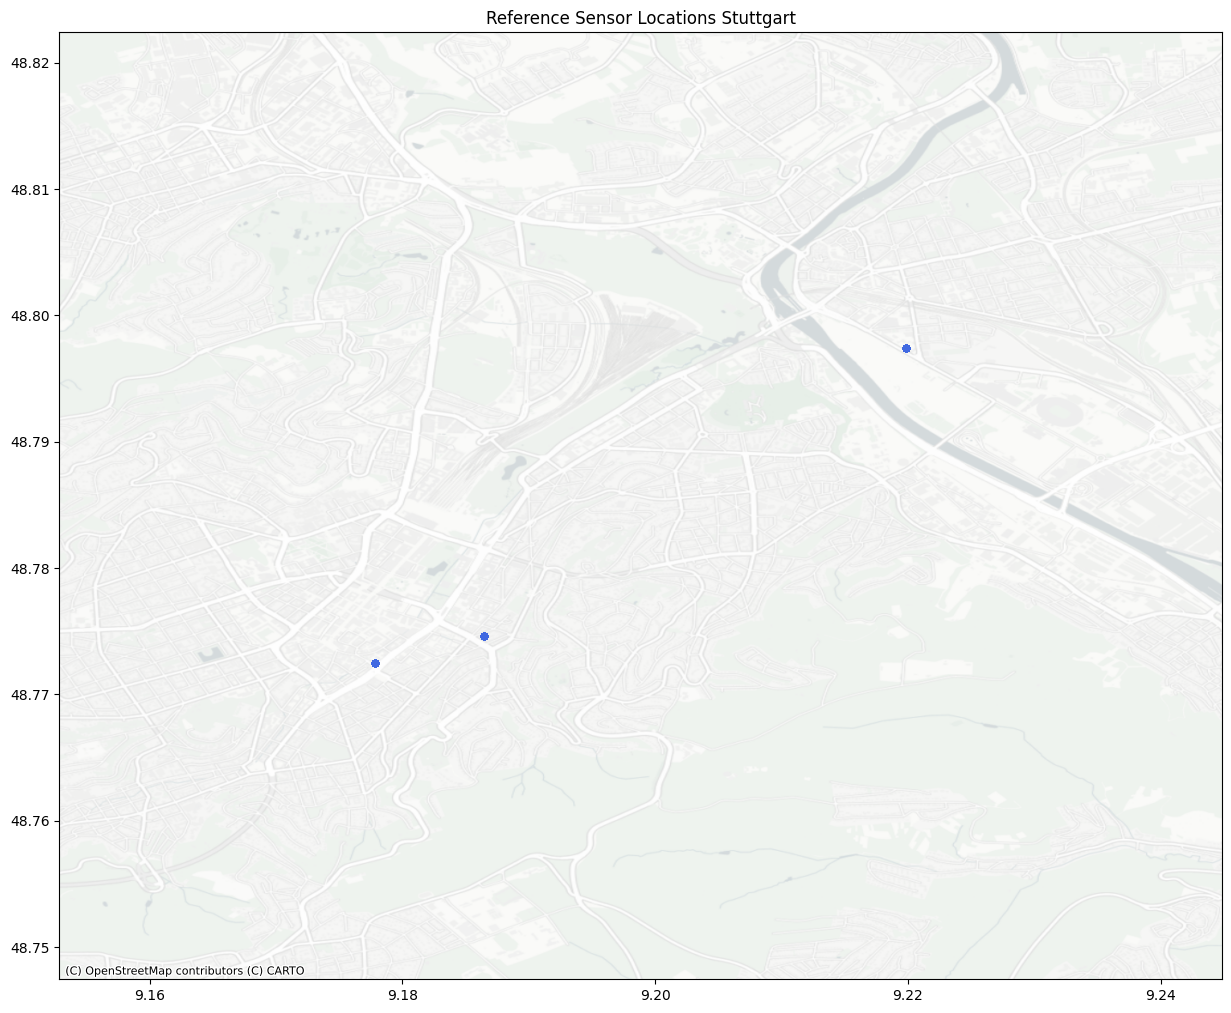
\includegraphics[width=1\textwidth]{images/afu_stuttgart_sensor_locations.png}
    \caption{Weather Station Locations in Stuttgart, \url{https://www.stadtklima-stuttgart.de/}, \textit{last accessed: 10.08.2023}}
    \label{fig:afu weather station locations}
\end{figure}

\subsubsection{City of Stuttgart – Office for Environmental Protection}

The Office for Environmental Protection of the city of Stuttgart has the goal of monitoring the climate in Stuttgart and the surrounding area and improve the living conditions of the citizens. The main focus of the office is on air quality, noise, and (urban) climate. It operates several weather stations in the city of Stuttgart, which are shown in Figure~\ref{fig:afu weather station locations}. The data from these stations is published directly on the website, a detailed quality assessment is given, and reference grade sensors are used. Unfortunately, the stations are mounted on top of building, e.g., 20-23m above ground, which is not ideal for measuring urban microclimates as the air temperature is several degrees cooler than directly on the ground. This example underlines the importance of proper sensor placement and meta-data documentation. The data from the weather stations could be corrected using the DWD reference station nearby, however uncorrected, the air temperature cannot be used to validate the crowdsourced data. Due to the high placement, other measurements such as wind direction and speed could be used to get a good estimation of the overall climate in the city, however not on the microscale.

\section{Remote Sensing Data Providers}

\subsubsection{Remote Sensing}
\label{subsec: remote sensing}

In comparison to stationary sensors that are installed directly in the environment they are observing, remote sensing describes the process of observing a target environment from afar~\cite{campbell2011introduction}. In climatology, remote sensing is used to collect meteorological data via satellites, planes, or balloons by either capturing image data that can be used to identify things like cloud and land coverage, by measuring passive radiation, or by actively sending out microwaves or using LiDAR to detect features such as surface temperature, e.g., LST data. Remote sensing comes with its own set of advantages and challenges.\\
The major upside of sensors moving way above ground is the high spatial coverage, that allows for meso- and planetary-scale analysis of weather phenomena. Another upside is the great data availability, as many satellite providers (e.g., NASA, ESA, etc.) publish their satellite data. This creates many research opportunities and services directly relying on these measurements.\\
Remote sensing also comes with certain downsides. The primary downside is the low spatio-temporal resolutions. Weather satellites usually are not orbit-stationary and move around earth on a predetermined orbit. Consequently, satellites only pass over each individual area a couple times a day, making real-time applications for currently unobserved areas impossible. Additionally, the spatial resolution can be too low for micro-/local-scale analysis, with typical LST resolution spanning from 1 km$^{2}$ to tens or even hundreds of km$^{2}$ per data point/grid field. In the atmosphere, there is also a lot of environmental noise, like radiation, that can have a negative influence on the measurement accuracy. Another disturbing factor can be clouds or other types of particles like rain that absorb radiation/microwaves sent from the sensors, making measuring under cloudy/rainy conditions either impossible. There exist methods to estimate values instead, relying on outgoing radiation from the surface, however these approaches are usually less accurate. These restrictions highly depend on the sensor used, as different sensors use different sensors use different technologies, e.g., microwaves with different wave lengths or higher resolution sensors.

\subsection{Google Earth Engine}

Google Earth Engine (Google EE) is a science data and analysis platform that allows users to work with and transform massive datasets with remote sensing data that are available as OpenSource~\cite{gorelick2017google}. Remote sensing data in this work is processed and obtained via this platform and used datasets are cited. Datasets available on Google EE are not published by Google itself but from institutions such as NASA, ESA, or the European Union.

\section{Quality Control}
\label{sec:quality control}

Quality control (QC) is an essential step in the process of data analysis and preparation. The goal is to identify and remove outliers in the data that are due to placement errors of sensors, sensor malfunctions, sensor inaccuracies or other errors. In the context of PWS, weather stations are placed and maintained by non-professionals, making QC even more important. One of the main challenges in the context of (hyper-) local urban air temperature data is to not flag data as outliers that is representative of the local climate in case of extreme temperature, e.g., heat islands, and at the same time identify erroneous or wrongly placed sensors, e.g., too close to walls, in direct sunlight, indoors, etc. Additionally, current PWS networks do not track sufficient metadata on the sensor placement, e.g., sensor height, which also plays an important role in protecting the privacy of citizens and not exposing too accurate sensor locations.\\
Due to the popularity of Netatmo weather station data in research due to high spatio-temporal resolution, there are several software libraries available that help simplify and automate the QC process. These tools were primarily developed for Netatmo temperature data, however CrowdQC and TITAN can also be used for other nearly-normally distributed data sources~\cite{hahn2022observations}. The following tools are available:

\begin{itemize}
    \item CrowdQC (R package~\footnote{\url{https://doi.org/10.14279/depositonce-6740.3}})
    \item CrowdQC+~\cite{fenner2021crowdqc+} (R package~\footnote{\url{https://github.com/dafenner/CrowdQCplus}})
    \item TITAN (R package~\footnote{\url{https://github.com/metno/TITAN}})
    \item NetatmoQC (Python 3 package~\footnote{\url{https://source.coderefinery.org/iOBS/wp2/task-2-3/netatmoqc}})
\end{itemize}

In this work, CrowdQC+ is used for QC as it offers improvements and bug fixes compared to CrowdQC. It's an open-source software library written in R, a popular programming language for statistical applications. The data needs to be in the following format:

\begin{itemize}
    \item \textit{p\_id}: The unique ID of the station
    \item \textit{time}: The time of the measurement
    \item \textit{ta}: The air temperature in degree Celsius
    \item \textit{lon}: The longitude of the station
    \item \textit{lat}: The latitude of the station
    \item \textit{z}: The height of the station in meters, optional
\end{itemize}

The CrowdQC+ library implements the following required steps of QC:\ Metadata Check, Distribution Check, Data Validity, Temporal Correlation, Spatial Buddy Check. There are also the following optional steps available, that are currently not used: Temporal Interpolation, Daily Validity, Validity in Time Period, and Correction for Time Constant.
The steps used in this work are shown and explained in Table~\ref{tab: qc_steps}, including the number of data and stations available after each step.\\
In their own study, CrowdQC+ kept 47.1\% and 69.2\% of data after steps m1-5, and only 20.7\% and 29.5\% after steps o1-o3, for the cities Amsterdam and Toulouse respectively~\cite{fenner2021crowdqc+}, given default parameters. In that setting, CrowdQC kept more data with 41.0\% in Amsterdam and 54.9\% in Toulouse. In this work, CrowdQC+ is used with default parameters excluding height validation, as this data was not available for almost all sensors. Additionally, only the first 5 required steps are used, as the optional steps are not needed for the interpolation. The input data for CrowdQC+ also needs have the same temporal resolution and intervals.\\
In this study, we use a 10 min interval to have a high temporal resolution and use the default parameters except excluding the heigh check due to the missing values. Important to note here, that in the following, only the air temperature is validated and no other measurements such as pressure or humidity. CrowdQC+ could be used for other approximately normally distributed features, however there hasn't been more specific research in this direction. We assume that a station that seems to be setup correctly and produces good air temperature measurements, also captures the other measurements correctly for simplicity reasons.

\begin{figure}[htp]
    \centering
    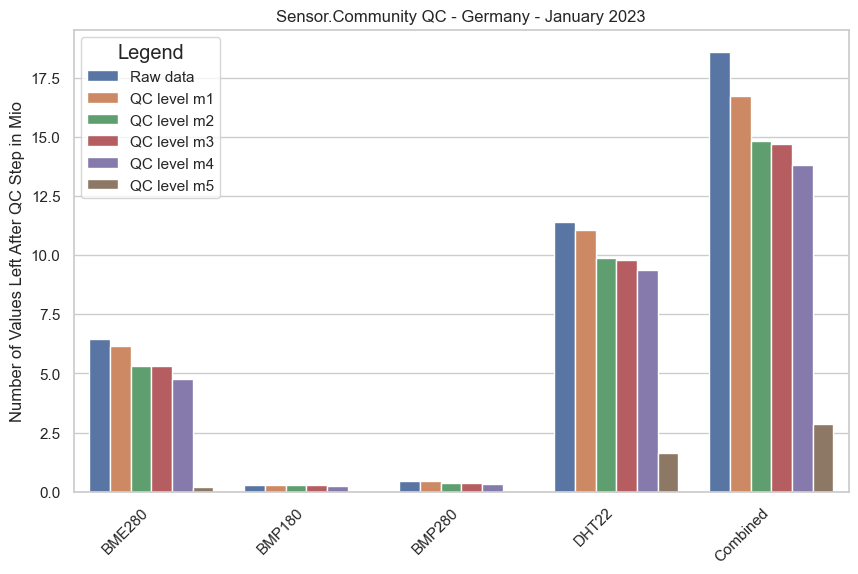
\includegraphics[width=1\textwidth]{images/sensor_community_qc_january_23.png}
    \caption{QC Results for Sensor.Community Data for Germany, January 2023}
    \label{fig:qc sensor community jan 23}

    \centering
    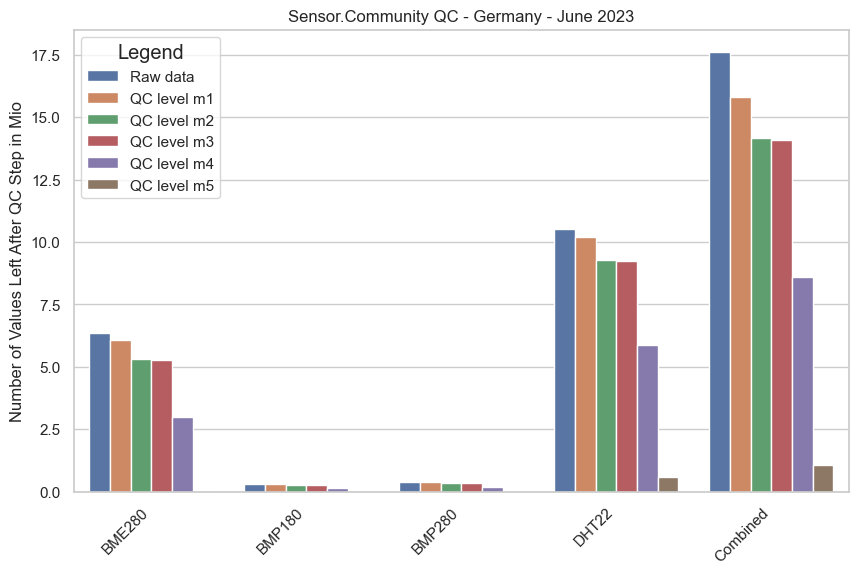
\includegraphics[width=1\textwidth]{images/sensor_community_qc_june_23.png}
    \caption{QC Results for Sensor.Community Data for Germany, June 2023}
    \label{fig:qc sensor community june 23}
\end{figure}

\subsection{Quality Control for Sensor.Community}

For Sensor.Community, we can see several interesting things for the air temperature. The first is, that in January 2023 less data is lost due to QC compared to June 2023. This could be to the fact, that in colder environments with less solar radiation, sensor placement, for example close to buildings, has less of an influence. In comparison, June 2023 had many hotter days, therefore it could be that more extreme readings are flagged as outliers. We can also see that Sensor.Community loses a lot of stations in step m4 in June 2023 compared to January 2023, which is the temporal correlation with the median of all stations. This could also be due to a higher temperature difference across Germany, therefore comparing smaller areas could be beneficial for this. We can also see, that the m5 check, which is the buddy check with surrounding stations, also removes a lot of stations which could be due to the low station density.\\
The CrowdQC+ library can theoretically be used to validate other near-normally distributed variables; however, this could change the way the QC step parameters should be set and changed from the default. For the air temperature, the default parameters as proposed by the library were used. Due to the limited scope, for other readings, e.g., relative humidity and atmospheric pressure, we simply remove default values. As an improvement, for other variables a more sophisticated QC process should be used. In addition, due to the low sensor density and the fact, that all types of sensors used are good low-cost sensors, we simply combine all sensor readings after QC step m5 into one dataset and ignore the sensor type.\\
After the QC process, the Sensor.Community sensor locations left are shown in~\ref{fig:qc sensor community germany june 23}. In this figure we can see, that there are many sensors left in Stuttgart, Hamburg, Munich, and some in Cologne. Due to DWD stations only being present in Hamburg and Stuttgart, those two areas are candidates for further usage.

\begin{figure}[ht]
    \centering
    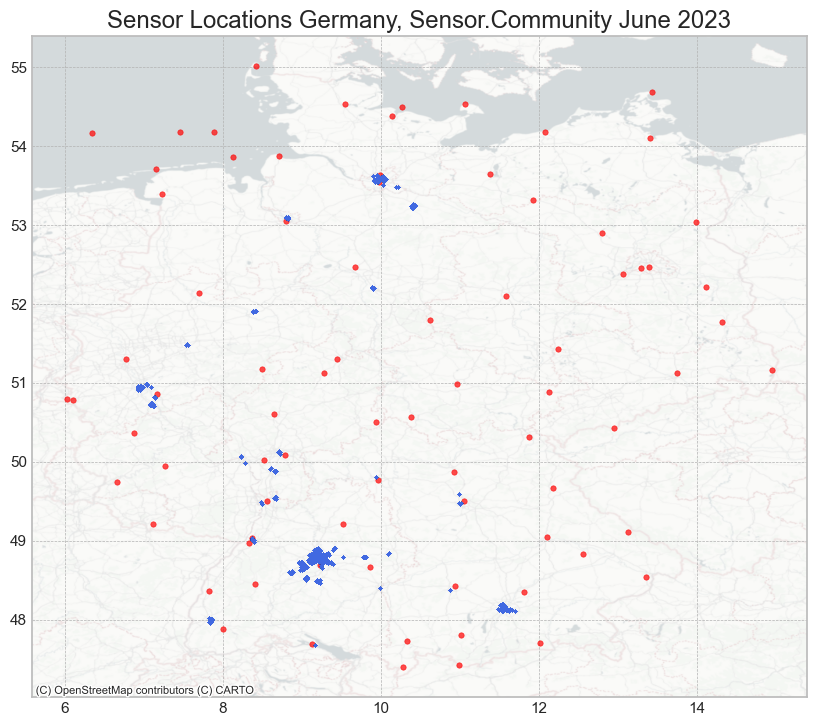
\includegraphics[width=1\textwidth]{images/sensor_community_locations_germany_after_qc_june_23.png}
    \caption{QC Results for Sensor.Community for Germany, June 2023}
    \label{fig:qc sensor community germany june 23}
\end{figure}

\begin{sidewaystable}
\label{tab: qc_steps}
\caption{Quality Control Steps of CrowdQC+}
\resizebox{\textwidth}{!}{
\begin{tabular}{lllllll}
\hline
\textbf{}         & \textbf{Id} & \textbf{Name of Step}        & \textbf{Functionality}                                                                                                                                                                                                                                                        & \textbf{\% of Data} & \textbf{Num Stations} & \textbf{Num Values} \\ \hline
\textbf{Required} &             &                              &                                                                                                                                                                                                                                                                               &                                                                                    &                                                                                         &                                                                  \\
                  & m1          & Metadata Check               & \begin{tabular}[c]{@{}l@{}}Validates longitude and latitude values and removes stations with\\ identical values. Mainly aims to remove stations with default values\\ from locations from IP addresses due to improper configuration\\ by the end-user\end{tabular}           & 97.40\%                                                                            & 1077                                                                                    & 2.082.283                                                        \\
                  & m2          & Distribution Check           & \begin{tabular}[c]{@{}l@{}}Primarily targets radiative error that lead to unrealistic high ta\\ values and sensors installed indoors\end{tabular}                                                                                                                             & 86.50\%                                                                            & 1041                                                                                    & 1.849.247                                                        \\
                  & m3          & Data Validity                & \begin{tabular}[c]{@{}l@{}}Checks values of stations that did not pass m2. If more than 20\%\\ of data didn't pass the check, the station is considered to be faulty\\ and is removed\end{tabular}                                                                            & 85.20\%                                                                            & 845                                                                                     & 1.821.479                                                        \\
                  & m4          & Temporal Correlation         & \begin{tabular}[c]{@{}l@{}}Checks the temporal correlation between each station and the\\ median of all stations for a specified period of time, default 1\\ month. Targets indoor stations that have weak temporal\\ correlation to the median of all stations.\end{tabular} & 79.90\%                                                                            & 829                                                                                     & 1.708.061                                                        \\
                  & m5          & Spatial Buddy Check          & \begin{tabular}[c]{@{}l@{}}Neighbourhood-based check to identify outliers within a specific\\ area. Primarily targets radiation errors with too high ta values.\\ Defaults to radius of 3000m and 5 neighbours.\end{tabular}                                                  & 31.53\%                                                                            & 466                                                                                     & 674.004                                                          \\
\textbf{Optional} &             &                              &                                                                                                                                                                                                                                                                               &                                                                                    &                                                                                         &                                                                  \\
                  & o1          & Temporal Interpolation       & \begin{tabular}[c]{@{}l@{}}Step to interpolate missing values in the time-series of each\\ station to increase data availability\end{tabular}                                                                                                                                 & -                                                                                  & -                                                                                       & -                                                                \\
                  & o2          & Daily Validity               & Verifies robust calculations of daily values                                                                                                                                                                                                                                  & -                                                                                  & -                                                                                       & -                                                                \\
                  & o3          & Validity in Time Period      & Checks if enough values are available in a given time frame                                                                                                                                                                                                                   & -                                                                                  & -                                                                                       & -                                                                \\
                  & o4          & Correction for Time Constant & \begin{tabular}[c]{@{}l@{}}Sensors have different times that they respond to ta changes.\\ Due to Netatmo design flaws, a\\ constant correction for all stations can be applied.\end{tabular}                                                                                 & -                                                                                  & -                                                                                       & -                                                                \\ \hline
\end{tabular}}
\vspace{1ex}

{\raggedright This table shows the QC steps used in this work from the CrowdQC+ library, including the \% of data available after each step, the number of stations available and the number of values left after each step. Optional steps are currently not used. \par}
\end{sidewaystable}

\begin{figure}[htp]
    \centering
    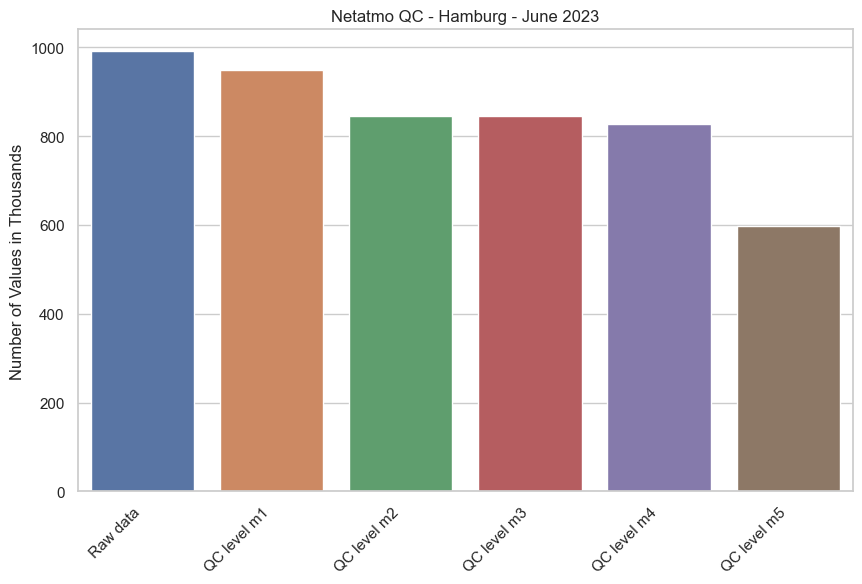
\includegraphics[width=1\textwidth]{images/netatmo_qc_june_23.png}
    \caption{QC Result Statistics for Netatmo Data for Hamburg, June 2023}
    \label{fig:qc netatmo june 23}
\end{figure}

\subsection{Quality Control for Netatmo}

The QC results for Netatmo stations in Hamburg during June 2023 can be found in~\ref{fig:qc netatmo june 23} which shows the absolute values of sensor readings available after each step including the overall available data as `Raw data' before QC which is 1.026.721 rows.
After QC 60.24\% of Netatmo data is still available in Hamburg (so a loss of 39.76\%). The amount of data kept is in line with comparable cities as tested by CrowdQC+'s study which kept 47.1\% and 69.2\% for the cities Amsterdam and Toulouse respectively after steps m1-m5~\cite{fenner2021crowdqc+} as mentioned above. Another comparison can be made to the study by Meier et al.\ which kept 47\% of Netatmo data in Berlin after QC with CrowdQC~\cite{meier2017crowdsourcing}.
It is interesting to note that stations directly next to water seem to be removed proportionally more often. This could be due to higher variability of wind close to water~\cite{ho2014mapping} which can result in higher prediction errors.\\
A station is not necessariliy removed at all times, only if it shows outliers for a certain period after QC step m3, maybe due to improper setup. The difference between day and night for an example day of 19.06.2023 can be found in Appendix~\ref{appendix: netatmo}  Figure~\ref{fig:qc netatmo hamburg before after m5}.

\section{Feature Engineering}
\label{sec:feature_engineering}

The goal of feature engineering is to create features from the available data that can be used as input for the machine learning models. Based on the features, different models can be used for completely different tasks such as interpolation vs.\ extrapolation. The process includes the selection of features, the extraction of features from the raw data, and the transformation of features into a format that can be used by the machine learning models which could include scaling and/or normalization. Especially in the context of air temperature interpolation, a lot of domain knowledge is required to select the right features and model correlations between them correctly. The target feature in this work is the air temperature at canopy height, e.g., 2m height so that CUHIs could be detected when using these trained interpolation models. Alternatively, the target temperature could also be adapted to be measured at another height or be exchanged based on the use-case.\\
The input features are a combination of sensor readings from PWS networks such as Sensor.Community and Netatmo, satellite data such as land cover and vegetation health or LST, and additional meta data such as soil conditions, zoning plans, or locations of sensors. The goal of this section is to give an overview of the different features that can be used for air temperature interpolation and discuss several highly important features that are especially relevant in the context of urban microclimate based on related studies. Important questions are: 1. What features are there and how can they be measured/sourced from? 2. How do features for the 2 use-cases, e.g., single station interpolation vs.\ areal interpolation, differ? 3. How do we handle QC outputs? 4. How do we deal with correlations between inputs so that we do not introduce bias into our models?

\subsection{Feature Engineering Pipelines and Automation}

Before looking at available features and features used in related work, we quickly return to the topic of Smart City and how to integrate different data sources and automate the feature engineering process. A popular solution for production-ready ML applications is the use of pipelines that streamline the data pre-processing, feature engineering, potential re-training, and prediction processes. Luckily, all data-sources previously mentioned have APIs or offer download options to get access to recent sensor readings. Next to the air temperature readings which can be sourced from Netatmo, Sensor.Community, and/or the DWD, other features are also important to get good prediction, as suggested by Zumwald et al.\ where air temperature at 2m only explained 33\% of the prediction~\cite{zumwald2021mapping}, such as remote sensing information, that for example could be sourced from Google EE.\\
The actual sensor readings come directly from the sensing layer, in which different external sources could be integrated via API, so that virtual sensors are created that are directly available for example via a overlay network such as SkipNet. In this work, we do not take advantage of other solutions but instead source data directly via API or archives to make a historical data analysis instead of testing real-time applications. After transporting this information via the transportation layer to the data-management layer, the service layer can consume the data streams. An air temperature interpolation service could then be placed in the service layer for areal interpolation. This service could then be used for areal interpolation to provide fine-granular air temperature maps/grids. The use-case of single station interpolation, for example in combination with moving sensors might be better located in the sensing layer as a virtual sensor, however challenges would be the dependency on other sensors which might have different sampling intervals.\\
In this work, we only take advantage of sklearn pipelines~\footnote{\url{https://scikit-learn.org/stable/modules/generated/sklearn.pipeline.Pipeline.html}, \textit{last accessed: 27.08.2023}} in a limited fashion for the actual training and testing process to automatically include scaling and cross-validation and rely on many manual steps to download the data, do pre-processing and QC, and finally extract features and train ML models.

\subsection{Feature Overview}

In the following sections, we look at available features for the use-case of air temperature interpolation.

\subsubsection{Essential Climate Variables}

Essential Climate Variables (ECV) are a list of currently 50 variables that are proposed by the WMO to measure climate and climate change. The WMO regularly publishes updates on which climate variables to use and how to measure them~\cite{wmo2018guide}. ECVs are generally more focused on measuring climate on a global scale, however they also contain many variables that are relevant for urban microclimate, such as air temperature and land cover. There are three categories of ECVs, namely Atmosphere, Land, and Ocean. And overview of the ECVs can be found online~\footnote{\url{https://gcos.wmo.int/en/essential-climate-variables/table}, \textit{last accessed: 08.08.2023}}.\\
Next to official WMO suggestions, other institutions such as the Integrated Climate Data Centre (ICDC) from the University of Hamburg (UHH) also suggest variables to measure climate~\footnote{\url{https://www.cen.uni-hamburg.de/icdc/data.html}, \textit{last accessed: 27.08.2023}}. Table~\ref{tab:icdc datset parameters} shows the available parameters for which datasets are available.

\begin{table}[ht]
    \footnotesize
    \centering
    \begin{tabular}{|c|c|}
        \hline
        \textbf{Category} & \textbf{Parameters} \\
        \hline
        \multirow{9}{*}{Atmospheric Data} & Air Temperature \\
        & Pressure \\
        & Wind \\
        & Precipitation \\
        & Clouds \\
        & Aerosols \\
        & Humidity \\
        & Radiation \\
        & Climate Indices \\
        \hline
        \multirow{7}{*}{Ocean} & Water Temperature \\
        & Wave Height (SSH) \\
        & Salt Content \\
        & Tide \\
        & Ocean Colour \\
        & Climatology \\
        & Ocean Currents \\
        \hline
        \multirow{8}{*}{Ice/Snow} & Sea Ice Coverage \\
        & Sea Ice Thickness \\
        & Sea Ice Type \\
        & Snow Thickness (Ice) \\
        & Snow Water Equivalent (SWE) \\
        & Land Snow Cover \\
        & Glacier Thickness \\
        & Melting Ponds \\
        \hline
        \multirow{7}{*}{Land} & Albedo \\
        & Surface Temperature \\
        & Vegetation \\
        & Soil Moisture \\
        & Topography \\
        & Short-wave Radiation \\
        & Permafrost \\
        \hline
        \multirow{1}{*}{Society} & Social Science Parameters \\
        \hline
    \end{tabular}
    \caption{ICDC Dataset Parameters}
    \label{tab:icdc datset parameters}
\end{table}

\begin{table}[htp]
    \footnotesize
    \centering
    \begin{tabular}{|lll|lll|}
    \hline
    \textbf{}                & \textbf{Variables (Units)}                                                                   & \multicolumn{1}{c}{\textbf{\begin{tabular}[c]{@{}c@{}}Acquisition\\ Source\end{tabular}}} & \textbf{}                & \textbf{Variables (Units)}                                                            & \multicolumn{1}{c|}{\textbf{\begin{tabular}[c]{@{}c@{}}Acquisition\\ Source\end{tabular}}} \\ \hline
    \rowcolor[HTML]{EFEFEF} 
                            & \textbf{Vegetation Index}                                                                    &                                                                                           &                          & \textbf{Radiation Index}                                                              &                                                                                            \\
                            & \begin{tabular}[c]{@{}l@{}}Normalized Difference Vegetation\\ Index (NDVI)\end{tabular}      & Landsat 8                                                                                 &                          & Spectral Radiance                                                                     & Landsat 8                                                                                  \\
                            & Enhanced Vegetation Index (EVI)                                                              & Landsat 8                                                                                 &                          & Emissivity                                                                            & Landsat 8                                                                                  \\
                            & \begin{tabular}[c]{@{}l@{}}Soil Adjusted Vegetation Index\\ (SAVI)\end{tabular}              & Landsat 8                                                                                 &                          & \begin{tabular}[c]{@{}l@{}}Tasseled Cap Transformation\\ Brightness\end{tabular}      & Landsat 8                                                                                  \\
                            & \begin{tabular}[c]{@{}l@{}}Tasseled Cap Transformation\\ Greenness (GVI)\end{tabular}        & Landsat 8                                                                                 & \cellcolor[HTML]{EFEFEF} & \cellcolor[HTML]{EFEFEF}\textbf{Building Index}                                       & \cellcolor[HTML]{EFEFEF}                                                                   \\
                            & Density of Low Vegetation                                                                    & LiDAR                                                                                     &                          & \begin{tabular}[c]{@{}l@{}}Normalized Difference Buit-Up\\ Index (NDBI)\end{tabular}  & Landsat 8                                                                                  \\
                            & Density of Medium Vegetation                                                                 & LiDAR                                                                                     &                          & Urban Index (UI)                                                                      & Landsat 8                                                                                  \\
                            & Density of High Vegetation                                                                   & LiDAR                                                                                     &                          & Index-based Built-Up Index (IBI)                                                      & Landsat 8                                                                                  \\
    \cellcolor[HTML]{EFEFEF} & \cellcolor[HTML]{EFEFEF}\textbf{Water Presence Index}                                        & \cellcolor[HTML]{EFEFEF}                                                                  &                          & Building Density                                                                      & LiDAR                                                                                      \\
                            & \begin{tabular}[c]{@{}l@{}}Modified Normalized Difference\\ Water Index (MNDWI)\end{tabular} & Landsat 8                                                                                 & \cellcolor[HTML]{EFEFEF} & \cellcolor[HTML]{EFEFEF}\textbf{Urban Morphology}                                     & \cellcolor[HTML]{EFEFEF}                                                                   \\
                            & \begin{tabular}[c]{@{}l@{}}Normalized Difference Water\\ Index (NDWI)\end{tabular}           & Landsat 8                                                                                 &                          & Sky View Factor                                                                       & LiDAR                                                                                      \\
    \cellcolor[HTML]{EFEFEF} & \cellcolor[HTML]{EFEFEF}\textbf{Bare Soil Index}                                             & \cellcolor[HTML]{EFEFEF}                                                                  &                          & \begin{tabular}[c]{@{}l@{}}Standard Deviation (STD) of\\ Building Height\end{tabular} & \begin{tabular}[c]{@{}l@{}}Local\\ Authority\end{tabular}                                  \\
                            & \begin{tabular}[c]{@{}l@{}}Normalized Difference Bareness\\ Index (NDBaI)\end{tabular}       & Landsat 8                                                                                 & \cellcolor[HTML]{EFEFEF} & \cellcolor[HTML]{EFEFEF}\textbf{Moisture Index}                                       & \cellcolor[HTML]{EFEFEF}                                                                   \\
                            & Bare Soil Index (BI)                                                                         & Landsat 8                                                                                 &                          & \begin{tabular}[c]{@{}l@{}}Tasseled Cap Transformation\\ Index\end{tabular}           & Landsat 8                                                                                  \\
                            & \begin{tabular}[c]{@{}l@{}}Enhanced Built-Up and Bareness\\ Index (EBBI)\end{tabular}        & Landsat 8                                                                                 &                          & \begin{tabular}[c]{@{}l@{}}Normalized Difference Moisture\\ Index (NDMI)\end{tabular} & Landsat 8                                                                                  \\
                            & Density of Bare Soil                                                                         & LiDAR                                                                                     &                          &                                                                                       &                                                                                            \\ \hline
    \end{tabular}
    \caption{Indexes used by Alonso and Renard~\cite{alonso2020new} to predict air temperature.}
    \label{tab:alonso_indexes}

    \begin{tabular}{|llll|}
    \hline
    \textbf{Variable}          & \textbf{Data source}                                                 & \textbf{Data type} & \textbf{Spatial resoltion} \\ \hline
    Red                        & \begin{tabular}[c]{@{}l@{}}Landsat 7,8 and\\ Sentinel 2\end{tabular} & Open source        & L: 30m, S: 10m             \\
    Green                      &                                                                      &                    &                            \\
    Blue                       &                                                                      &                    &                            \\
    Near infrared              &                                                                      &                    &                            \\
    Short-wave infrared 1      &                                                                      &                    & L: 30m, S: 20m             \\
    Short-wave infrared 2      &                                                                      &                    &                            \\
    NDVI                       &                                                                      &                    & L: 30m, S: 10m             \\
    IBI                        &                                                                      &                    & L: 30m, S: 20m             \\
    LST                        & Landsat 7,8                                                          &                    & 30m                        \\
    Elevation above sea        & STRM                                                                 &                    & 30m                        \\
    Terrain aspect             &                                                                      &                    &                            \\
    Terrain slope              &                                                                      &                    &                            \\
    Terrain ruggedness         &                                                                      &                    &                            \\
    CHM                        & LiDAR                                                                & Closed source      & 1m                         \\
    CHM slope                  &                                                                      &                    &                            \\
    CHM aspect                 &                                                                      &                    &                            \\
    CHM shadow/SVI             &                                                                      &                    &                            \\
    Building height            & \begin{tabular}[c]{@{}l@{}}LiDAR + building\\ footprint\end{tabular} &                    &                            \\
    Building height sd 1-4m    &                                                                      &                    &                            \\
    Building height sd 4-20m   &                                                                      &                    &                            \\
    Building height sd 20-100m &                                                                      &                    &                            \\
    Fractional tree cover      & \begin{tabular}[c]{@{}l@{}}LiDAR + ortho-\\ photo\end{tabular}       &                    &                            \\
    Tree height                &                                                                      &                    &                            \\
    Distance to coast          & Global water occurrence                                              & Open source        & 30m                        \\
    Distance to fresh water    &                                                                      &                    &                            \\ \hline
    \end{tabular}
    \caption{Features for Air Temperature Interpolation used by Venter et al.~\cite{venter2020hyperlocal}}
    \label{tab: venter features interpolation}
\end{table}

\subsubsection{Features used in Related Work}

Related studies can give a good overview of which features work best for air temperature interpolation. The used features can be roughly divided into 4 categories: raw in-situ measurements, raw satellite data, calculated features, and additional meta data. An important way to use satellite data is to calculate indexes out of the raw data. Alonso and Renard~\cite{alonso2020new} used among other data the indexes shown in Table~\ref{tab:alonso_indexes} to predict air temperature. These indexes are either available as precalculated datasets or can be calculated from raw satellite data. Especially the Google Earth Engine platform provides a lot of precalculated datasets from various sources such as MODIS~\cite{didan2021modis}; however, each index is separately available, therefore requiring some work to combine them into a single dataset. Due to the interference from clouds, these indexes usually also include quality bands, which indicate the quality of the index value for a given pixel, as well as missing values.\\
In comparison to MODIS, Sentinel satellite data provides a significantly higher resolution at 10-60 m$^2$ per pixel compared to 500-1000 m$^2$ per pixel for MODIS but there are no precalculated indexes available for Sentinel data on the Google Earth Engine platform.\\
However, there exist scripts published by other researchers to manually calculate such indexes for example the NDVI index from Sentinel data by the Free University of Berlin~\footnote{\url{https://www.geo.fu-berlin.de/en/v/geo-it/gee/2-monitoring-ndvi-nbr/2-2-calculating-indices/ndvi-s2/index.html}, \textit{last accessed: 09.08.2023}}.\\
In comparison to MODIS and Sentinel, many LiDAR datasets are closed source and are not available for research purposes. This is unfortunate as LiDAR data provides a very high resolution of 5-10 cm$^2$ per pixel and enables the capturing of detailed elevation data. Especially in the context of urban areas and building heights this information can be very useful, for example to calculate the sky view factor which seems to have a significant impact on air temperature modelling~\cite{dirksen2019sky}.\\
Next to index data from remote sensing, there are also other types of information that could be useful for ML applications. Alonso and Renard~\cite{alonso2020new} also used the following information:

% Todo: make into table on one page
\begin{itemize}
    \item Topographic

    \begin{itemize}
        \item Slope (°)
        \item Exposure
        \item Curvature
    \end{itemize}
    \item Land use

    \begin{itemize}
        \item Distance to railway tracks
        \item Distance to points of tourist interest
        \item Distance to subway entrances
        \item Distances to fountains
        \item Water area
    \end{itemize}
\end{itemize}

For the hyperlocal air temperature mapping study done in Oslo by Venter et al.~\cite{venter2020hyperlocal}, the used features are shown in Table~\ref{tab: venter features interpolation}.

\subsection{Features used in this Work}

In the following, we describe which features are used in this work for our two use-cases, e.g., single station interpolation and areal interpolation. Due to the limited scope of this work, only a subset of the available features will be used to show the feasibility of the respective use-case and get an idea on the upper bounds of RMSE values that can be expected when choosing one of the use-cases, as we expect that with an increase of features and therefore availability of information for the ML models to learn from, the prediction quality will increase.

\subsubsection{Features for Areal Interpolation}

\begin{table}[ht]
    \footnotesize
    \centering
    \begin{tabular}{|lll|}
    \hline
    Measurement (Units)                                                 & Spatial Resolution & Temporal Resolution                                                                                                                    \\ \hline
    \rowcolor[HTML]{EFEFEF} 
    \textbf{Weather Station/Sensor Measurements}                        &                    &                                                                                                                                        \\
    \begin{tabular}[c]{@{}l@{}}Air temperature (°C)\\ Mean\end{tabular} & Single location    & \begin{tabular}[c]{@{}l@{}}10 min (Sensor.Community)\\ 10 min (DWD)\\ 30 min (Netatmo Historical)\\ 10 min (Netatmo Live)\end{tabular} \\
    Relative Humidity (\%)                                              & Single location    & \begin{tabular}[c]{@{}l@{}}10 min (Sensor.Community)\\ 10 min (DWD)\\ 30 min (Netatmo Historical)\\ 10 min (Netatmo Live)\end{tabular} \\
    Atmospheric Pressure (mBar)                                         & Single location    & \begin{tabular}[c]{@{}l@{}}10 min (Sensor.Community)\\ 10 min (DWD)\\ 30 min (Netatmo Historical)\\ 10 min (Netatmo Live)\end{tabular} \\
    Wind Strength (km/h)                                                 & Single location    & \begin{tabular}[c]{@{}l@{}}10 min (Sensor.Community)\\ 10 min (DWD)\\ 30 min (Netatmo Historical)\\ 10 min (Netatmo Live)\end{tabular} \\
    Wind Direction (°)                                                  & Single location    & \begin{tabular}[c]{@{}l@{}}10 min (Sensor.Community)\\ 10 min (DWD)\\ 30 min (Netatmo Historical)\\ 10 min (Netatmo Live)\end{tabular} \\
    Precipitation (mm)                                                  & Single location    & \begin{tabular}[c]{@{}l@{}}10 min (DWD)\\ 30 min (Netatmo Historical)\\ 10 min (Netatmo Live)\end{tabular}                             \\
    \rowcolor[HTML]{EFEFEF} 
    \textbf{Remote Sensing Data}                                        &                    &                                                                                                                                        \\
    NDVI (MODIS)                                                        & 500m               & 16 days                                                                                                                                \\
    EVI (MODIS)                                                         & 500m               & 16 days                                                                                                                                \\
    DEM (Copernicus)                                                    & 30m                & 2015 - 2017                                                                                                                            \\ \hline
    \end{tabular}
    \caption{Features for Air Temperature Interpolation Used in this Work}
    \label{tab:features this work}
\end{table}

Air temperature, relative humidity, atmospheric pressure, precipitation, and wind was sourced from Netatmo and Sensor.Community PWS networks as well as the DWD weather stations as reference data.
All remote sensing data acquired in this work was processed using the Google Earth Engine~\cite{gorelick2017google} as it offers a unified way of accessing data and offers enhanced processing capabilities that are especially important when dealing with these large datasets that can grow as large as several hundred terabytes. The following datasets have been used and downloaded from the Google Earth Engine platform:

\begin{itemize}
    \item MODIS/061/MOD13A1: MODIS Vegetation Indexes NDVI and EVI\\
    (500m, 16 days)~\cite{didan2021modis}
    \item COPERNICUS/DEM/GLO30: Copernicus Digital Elevations Model (30m)~\cite{copernicus30dem}
\end{itemize}

Potential datasets that could be used in the future are:

\begin{itemize}
    \item MODIS\_061\_MOD15A2H: MODIS Leaf Area Index/FPAR \\
    (500m, 8 days)~\cite{myneni2021modis}
    \item COPERNICUS\_S2\_SR: Sentinel-2 Multi Spectral Instrument, Level-2A\\
    (10m, 5 days)~\cite{sentinel2msi} (for manual index calculation)
\end{itemize}

Additionally, location data was incorporated into the models by longitude and latitude values in coordinate reference system EPSG:4326. As noted by Hengl et al.\ this might not be optimal~\cite{hengl2018random} and could be improved by using distances between sampling locations instead. The features used in this work are shown in Table~\ref{tab:features this work} and were chosen based on availability and relevance for air temperature modelling. The number of features in the initial scope of this work is quite limited and could be increased to gain better prediction results.

\subsubsection{Features for Single Station Interpolation}

For the single station interpolation use-case, we keep the setup rather simple. The idea behind this approach is the hypothesis that the model does not really care about the location of the sensor, but only about the similarity in temperature curves. Therefore, we use the air temperature readings of neighbouring sensors as covariants ordered by the distance to the sensor and always in the same order. Next to the air temperature, we also include the humidity and pressure of neighbours as covariants in the same order, and the time of the reading converted to a sinus function, so that we can explore if the time of day has an influence on prediction errors as shown in Appendix~\ref{lst: timestamp to sin}.

\section{Additional Considerations}
\label{sec: additional considerations}

Next to the features, there are also additional considerations when creating train and test datasets. These include sampling, normalization, and scaling, dealing with correlations, and more. If your model for example expects uncorrelated input variables, one could calculate the variance inflation factor (VIF) to make sure the input variables are uncorrelated. If the VIF is over 10~\cite{montgomery2021introduction} or more restrictive over 3~\cite{zuur2010protocol}, this indicates that the model is invalid. Another option could be principal component analysis (PCA) to turn correlated variables into new uncorrelated ones. In this work, we try to choose models which can deal with correlations naturally like RF, so we reduce the complexity of working with this type of features.\\
Other considerations include imputation for missing values and feature scaling. These will be covered in the evaluation where appropriate, as some models such as KNN need feature scaling, while others such as RF or HGB do not need scaling, as all models except HGB cannot handle missing values and need imputation.

\subsubsection{Spatial Autocorrelation}

Spatial autocorrelation is the presence of `systematic spatial variation in a mapped variable'~\cite{haining2001spatial}. If adjacent variables tend to have similar values, spatial autocorrelation is positive. In contrast if adjacent variables tend to have very contrasting values, the spatial autocorrelation is negative. It can be defined traditionally via the Moran's I index~\cite{moran1948interpretation} or the Geary's coefficient~\cite{geary1954contiguity}. The goal of using ML in this context would be that these correlations can be ignored, simplifying the interpolation process. Especially in geostatistical methods such as Kriging, not dealing with correlations can lead to wrong interpolations and the introduction of bias.\\

\subsubsection{Temporal Autocorrelation}

Next to spatial autocorrelations, there can also be temporal autocorrelations between successive values of the same variable. Also, there can be seasonal trends that might need to be corrected, as well as temporal lag. In the case of temperature sensors, this could relate to the time it takes for a sensor to adjust to a new temperature. A reference-grade sensor might adjust in a few seconds, where a LCS might need more time. Especially with Netatmo sensor which have a suboptimal ventilation and small form factor, this could mean that after they heated up, they need more time to cool down again, resulting in a bias towards longer hotter temperatures.
